%%%%%%%%%%%%%%%%%%%%%%%%%%%%%%%%%%%%%%%%%%%%%%%%%%%%%%%%%%%%%%%%%%%%%%
% Lớp 10 | Mệnh đề. Tập hợp | Tập hợp
% Dạng 0D1?2-3: Ký hiệu khoảng, đoạn, nửa khoảng
% Số câu: 20  (sinh tự động bởi tach_cau.py; từ nay thầy sửa trực tiếp file này)
%%%%%%%%%%%%%%%%%%%%%%%%%%%%%%%%%%%%%%%%%%%%%%%%%%%%%%%%%%%%%%%%%%%%%%

%%%%%%%%%%%%%%%% TRẮC NGHIỆM 4 PHƯƠNG ÁN %%%%%%%%%%%%%%%%

% nguồn: MaHoaNH_TracNghiem_Lop10
\begin{ex}%[0D1N2-3]%[ma:1bb188d0]
	Kí hiệu nào sau đây dùng để viết  đúng mệnh đề \lq\lq~$\sqrt{2}$ không phải là số hữu tỉ~\rq\rq?
	 \choice
		{$\sqrt{2}\subset \mathbb{Q}$} 
		{\True $\sqrt{2}\notin \mathbb{Q}$} 
		 {$\sqrt{2}\ne \mathbb{Q}$}
		{$\sqrt{2}\in  \mathbb{Q}$}
	 \loigiai{
	Cách  viết đúng là $\sqrt{2} \notin \mathbb{Q}$.}
\end{ex}

% nguồn: MaHoaNH_TracNghiem_Lop10
\begin{ex}%[0D1N2-3]%[ma:34fdbdaf]
	Sử dụng kí hiệu khoảng, nửa khoảng, đoạn để viết tập hợp $A=\left\{x\in\mathbb{R}\left|-3 <  x\le 5\right.\right\}$.
	 \choice
		{$A=\left\{-2;-1;0;1;2;3;4;5\right\}$} 
		{\True $A=(-3;5]$} 
		{$A=[-3;5)$} 
		 {$A=[-3;5]$}
	 \loigiai{
	Theo định nghĩa các tập  con của tập số thực thì $A=(-3;5]$.}
\end{ex}

% nguồn: MaHoaNH_TracNghiem_Lop10
\begin{ex}%[0D1N2-3]%[ma:3dbaae9e]
	Tập $A=\{0;1;2\}$ có  bao nhiêu tập con có đúng $2$ phần tử?
	 \choice
		 {$6$}
		{$7$} 
		 {\True $3$}
		 {$4$}
	\loigiai{ 
		Có $3$ tập  con có đúng $2$ phần tử của tập $A=\left\{ 0;1;2 \right\}$ là $\left\{ 0;1 \right\}$, $\left\{ 0;2 \right\}$, $\left\{ 1;2 \right\}$.
	} 
\end{ex}

% nguồn: MaHoaNH_TracNghiem_Lop10
\begin{ex}%[0D1N2-3]%[ma:78248ca7]
	Cho tập $A$ có $3$ phần tử,  số tập con của tập $A$ bằng
	\choice 
		 {$6$}
		{$3$} 
		 {\True $8$}
		{$4$} 
	\loigiai{ 
		Giả sử $A=\left\{  a;b;c \right\}$, các tập con của $A$ là: $\varnothing$, $\left\{ a \right\}$, $\left\{ b \right\}$, $\left\{ c \right\}$, $\left\{ a;b \right\}$, $\left\{ a;c \right\}$, $\left\{ b;c \right\}$, $\left\{ a;b;c \right\}$.\\
	Vậy có $8$ tập con của  $A$.}
\end{ex}

% nguồn: MaHoaNH_TracNghiem_Lop10
\begin{ex}%[0D1N2-3]%[ma:0e98783e]
	Có bao nhiêu tập  $A$ để $\left\{ m;n \right\}\subset A\subset \left\{ m;n;x;y \right\}$ ?
	 \choice
		 {$2$}
		{\True  $4$}
		 {$1$}
		 {$3$}
	\loigiai{ 
		Vì $\{ m;n \}  \subset A \subset \{ m;n;x;y \}$nên $A$ có thể là một trong bốn tập hợp sau
		 \[
		\{ m;n  \};~\{m;n;x\};~\{ m;n;y \};~\{ m;n;x;y\}.
		\] 
	} 
\end{ex}

% nguồn: MaHoaNH_TracNghiem_Lop10
\begin{ex}%[0D1N2-3]%[ma:08649e4d]
	Cho tập $A=\{ x\in \mathbb{N}|~(2-x)(x^2-3x-4)=0  \}$. Hỏi tập $A$ có bao nhiêu tập con ?
	\choice 
		 {$2$}
		{\True  $4$}
		{$7$} 
		 {$8$}
	\loigiai{ 
		 Ta có $(2-x)(x^2-3x-4)=0 \Leftrightarrow \hoac{
		& x=2  \in \mathbb{N} \\
		& x=-1 \notin \mathbb{N} \\ 
		& x=4  \in \mathbb{N}.}$\\
		Vậy $A=\{ 2;4 \}$ nên $A$ có các tập con là $\{ 2\}$; $\{ 4\}$; $\{  2;4\}$; $\varnothing$.
	 }
\end{ex}

% nguồn: MaHoaNH_TracNghiem_Lop10
\begin{ex}%[0D1N2-3]%[ma:042d1746]
	 Cho tập $X=\{ x \in \mathbb{N} |~ (x^2-4)(x-1)=0\}$. Tính số phần tử của $X$.
	 \choice
		 {$1$}
		{$3$} 
		 {\True $2$}
		 {$4$}
	 \loigiai{
		Ta  có
		 \[
		(x^2-4)(x-1)=0 
		\Leftrightarrow \hoac{&x^2-4=0\\&x-1=0} 
		\Leftrightarrow \hoac{&x=2\\&x=-2 \notin \mathbb{N}\\&x=1.} 
		 \]
		Do $x\in \mathbb{N}  \Rightarrow x \in \{ 2;1\}$. Vậy $X$ có $2$ phần tử.
	 }
\end{ex}

% nguồn: MaHoaNH_TracNghiem_Lop10
\begin{ex}%[0D1N2-3]%[ma:a08f1641]
	Cho tập hợp  $A=\{ x \in \mathbb{N} |~(x-1)(2x+4)=0 \}$. Tập $A$ được viết theo kiểu liệt kê là
	 \choice
		 {$\{ -1;4 \}$}
		{\True $\{  1 \}$}
		{$\{ 1;-2 \}$} 
		 {$\{ -1;-2 \}$}
	 \loigiai{
		Ta có 
		\[ 
		(x-1)(2x+4)=0 
		\Leftrightarrow  \hoac{&x-1=0\\&2x+4=0}
		\Leftrightarrow \hoac{&x=1\\&x=-2 \notin  \mathbb{N}.}
		\] 
		Vậy $A=\{ x \in \mathbb{N} |~ (x-1)(2x+4)=0  \} = \{ 1 \}$.
	 }
\end{ex}

% nguồn: MaHoaNH_TracNghiem_Lop10
\begin{ex}%[0D1N2-3]%[ma:71f471ad]
	Viết tập hợp $A=\{ x \in \mathbb{N} |~ (2x+1)(x^2-5x+6)=0\}$ bằng  cách liệt kê.
	\choice 
		{$\{ -1;2;3  \}$}
		{\True $\{  2;3 \}$}
		 {$\left\{ -\dfrac{1}{2};2;3 \right\}$}
		{$\{ -1;2 \}$} 
	 \loigiai{
		Ta có 
		\[ 
		(2x+1)(x^2-5x+6)=0  \Leftrightarrow
		\hoac{&2x+1=0\\&x^2-5x+6=0} \Leftrightarrow 
		 \hoac{&x=-\dfrac{1}{2}\\&x=2\\&x=3.}
		\] 
		Do $x \in  \mathbb{N} \Rightarrow A=\left\{ 2;3 \right\}$.
	 }
\end{ex}

% nguồn: MaHoaNH_TracNghiem_Lop10
\begin{ex}%[0D1N2-3]%[ma:b26dadc3]
	Trong các tập hợp sau, tập nào là  tập rỗng?
	 \choice
		 {$A= \{ x \in \mathbb{R} |~ x^2+5x-6=0 \}$}
		{$B=\{  x \in \mathbb{Q} |~ 3x^2-5x+2=0 \}$}
		{\True $C=\{ x\in \mathbb{Z} |~ x^2+x-1=0  \}$}
		{$D=\{ x \in \mathbb{R} |~ x^2+5x-1=0 \}$} 
	 \loigiai{
		Ta có\\ 
		 $x^2+5x-6=0
		\Leftrightarrow \hoac{&x=1 \in \mathbb{R}\\&x=-6 \in \mathbb{R}}$. Vậy $A=\{ -6;1  \} \neq \varnothing$.\\
		$3x^2-5x+2=0 
		\Leftrightarrow \hoac{&x=1 \in \mathbb{Q}\\&x=\dfrac{2}{3} \in \mathbb{Q}}$. Vậy $B=\left\{ 1;\dfrac{2}{3}  \right\} \neq \varnothing$.\\
		 $x^2+x-1=0
		\Leftrightarrow \hoac{&x=\dfrac{-1+\sqrt{5}}{2} \notin \mathbb{Z}\\&x=\dfrac{-1-\sqrt{5}}{2} \notin \mathbb{Z}}$. Vì $x \in \mathbb{Z}$  nên $C=\varnothing$.\\
		$x^2+5x-1=0 
		\Leftrightarrow \hoac{&x=\dfrac{-5+\sqrt{29}}{2} \in \mathbb{R}\\&x=\dfrac{-5-\sqrt{29}}{2} \in \mathbb{R}}$.  Vậy $D=\left\{ \dfrac{-5+\sqrt{29}}{2};\dfrac{-5-\sqrt{29}}{2} \right\} \neq \varnothing$.
	} 
\end{ex}

% nguồn: MaHoaNH_TracNghiem_Lop10
\begin{ex}%[0D1H2-3]%[ma:e60745e5]
	Tìm tất cả các giá trị của  tham số $m$ sao cho $(m;+\infty)\subset(1;+\infty)$?
	 \choice
		{$m<1$} 
		 {$m\leq 1$}
		{\True $m\geq 1$} 
		 {$m>1$}
	 \loigiai{
		Do $(m;+\infty)\subset(1;+\infty)$  nên $m\geq 1$.
	} 
\end{ex}

% nguồn: MaHoaNH_TracNghiem_Lop10
\begin{ex}%[0D1H2-3]%[ma:129f0ffa]
	Liệt kê các phần tử của tập hợp $A=\{ x \in \mathbb{Z}|~ (6x^2-7x+1)(x^2-4)=0\}$ ta được 
	\choice 
		 {$A=\left\{\dfrac{1}{6};\dfrac{1}{2};2 \right\}$}
		{\True  $A=\{-2;1;2\}$}
		{$A=\left\{-2;\dfrac{1}{6};1;2  \right\}$}
		 {$A=\{1;2\}$}
	\loigiai{ 
		Xét  phương trình
		\[ 
		(6x^2-7x+1)(x^2-4)=0  \Leftrightarrow
		 \hoac{&6x^2-7x+1=0\\&x^2-4=0} \Leftrightarrow
		\hoac{&x=1 \in \mathbb{Z}\\&x=\dfrac{1}{6} \notin \mathbb{Z}\\&x = 2  \in \mathbb{Z}\\& x=-2 \in \mathbb{Z}.}
		 \]
	Vậy  $A=\{-2;1;2\}.$}
\end{ex}

% nguồn: MaHoaNH_TracNghiem_Lop10
\begin{ex}%[0D1H2-3]%[ma:8406377b]
	Cho $A=[-1;  3]$; $B=(2; 5)$. Tìm mệnh đề \textbf{sai}.
	 \choice
		{$B \setminus  A=(3; 5)$}
		{$A \cap  B=(2; 3]$}
		{$A \setminus  B=[-1; 2]$}
		{\True $A \cup B=[-1; 5]$} 
	\loigiai{ 
		\begin{center}
			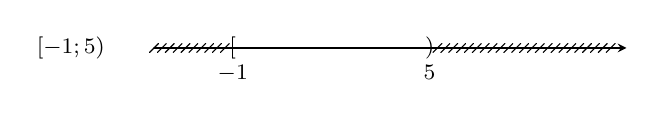
\begin{tikzpicture}[scale=1,>=stealth,font=\footnotesize,line join=round,line cap=round]
					\draw [-stealth]  (0,0)--(6,0);
					 \path (1,0) node{$[$}
						(1,-0.1) node[below]{$-1$} 
						 (-.5,0) node[left]{$[-1; 5)$};
					 \path (3.5,0) node{$)$}
						 (3.5,-0.1) node[below]{$5$};
					\foreach \x in{0,0.1,...,1}  \draw (\x,0)--++(45:.08)
						 (\x,0)--++(-135:.08);
					 \foreach \x in{3.6,3.7,...,5.8} \draw (\x,0)--++(45:.08)
						 (\x,0)--++(-135:.08);
				\end{tikzpicture}
		\end{center}
		Ta có $A \cup B=[-1; 5)$. 
	 }
\end{ex}


%%%%%%%%%%%%%%%% ĐÚNG/SAI %%%%%%%%%%%%%%%%

% nguồn: MaHoaNH_DungSai_Lop10
\begin{ex}%[0D1N2-3]%[ma:1339923e]
	Cho hai tập  hợp $A=\{x\in \mathbb{R}|~(x-1)(x-2)(x-3)=0\}$, $B=\{5;3;1\}$.
	 \choiceTF
		{\True Tập hợp $A$  có $3$ phần tử}
		{Tập hợp $A\cup B$ có $6$ phần tử} 
		{Tập hợp $A  \subset B$}
		{Tập hợp $B \subset  A$}
	 \loigiai{
		\begin{itemchoice}
			 \itemch
			Ta có $(x-1)(x-2)(x-3)=0  \Leftrightarrow
			 \hoac{&x-1=0\\&x-2=0\\&x-3=0} \Leftrightarrow
			 \hoac{&x=1\\&x=2\\&x=3.}$\\
			Do  vậy $A=\{2; 3; 1\}$.
			 \itemch
			Ta  có $A\cup B =\{ 1;2;3;5\}$. Vậy $A\cup B$ có $4$ phần tử.
			 \itemch
			Ta có $2 \in A$ nhưng $2 \notin B$ nên $A$ không là tập con  của $B$.
			 \itemch
			Ta có $5 \in B$ nhưng $5 \notin A$ nên $B$ không là  tập con của $A$.
		\end{itemchoice}
	 }
\end{ex}

% nguồn: MaHoaNH_DungSai_Lop10
\begin{ex}%[0D1H2-3]%[ma:5e4e0f3a]
	Lớp $10C6$ có $18$ học sinh tham gia câu lạc bộ bóng đá và $15$ học sinh tham gia câu lạc bộ bóng rổ. Biết rằng có $10$ học sinh tham gia cả hai câu lạc  bộ trên. Khi đó
	 \choiceTF
		{\True Có $8$ học sinh tham gia ít nhất một trong hai  câu lạc bộ trên}
		{\True Có $23$ học sinh tham gia ít nhất một  trong hai câu lạc bộ trên}
		{Biết lớp $10C6$ có $45$ học sinh. Có $25$ học  sinh không tham gia câu lạc bộ bóng đá}
		{Biết lớp $10C6$ có $45$ học sinh. Có $24$ học sinh không tham  gia cả hai câu lạc bộ}
	\loigiai{ 
		Gọi $A$, $B$, $E$ lần lượt là tập hợp các học sinh của lớp tham gia câu lạc bộ bóng đá, câu lạc bộ bóng  rổ và học sinh lớp $10C6$.\\
		Khi đó $A \cap B$ là tập hợp học sinh tham gia cả hai câu lạc bộ và $|A \cap B|=10$. Số  phần tử của $A$ là $|A|=18$, số phần tử của $B$ là $|B|=15$.
		\begin{itemchoice}
			\itemch Tập hợp các học sinh tham  gia câu lạc bộ bóng đá và không tham gia câu lạc bộ bóng rổ là tập hợp $A\setminus B$. Số phần tử của $A\setminus B$ chính là số phần tử của $A$ trừ đi số phần tử của $A \cap B$.\\
			Vậy số học sinh tham gia câu lạc bộ bóng đá và không tham  gia câu lạc bộ bóng rổ là $18-10=8$ (học sinh).
			\itemch Tập hợp các học sinh tham gia ít nhất một trong hai câu  lạc bộ trên chính là tập hợp $A \cup B$. Do khi đếm số học sinh tham gia câu lạc bộ bóng đá là $18$, số học sinh tham gia câu lạc bộ bóng rổ là $15$ thì số học sinh tham gia cả hai câu lạc bộ là $10$ được tính hai lần.\\
			Vậy số học sinh  tham gia ít nhất một trong hai câu lạc bộ trên là $18+15-10=23$ (học sinh).
			\itemch Số phần tử  của $E$ là $45$. Tập hợp các học sinh không tham gia câu lạc bộ bóng đá là phần bù của $A$ trong $E$.\\
			Vậy số học sinh không tham gia câu lạc bộ bóng đá là $45-18=27$ (học sinh). 
			\itemch Tập hợp các học sinh không  tham gia cả hai câu lạc bộ là phần bù của $A \cup B$ trong $E$.\\
			Vậy số học sinh  không tham gia cả hai câu lạc bộ là $45-23=22$ (học sinh).
		\end{itemchoice}
	} 
\end{ex}

% nguồn: MaHoaNH_DungSai_Lop10
\begin{ex}%[0D1H2-3]%[ma:0b912f6c]
	Cho các tập hợp $G=\left\{\left. x\in \mathbb{R}\right|-12\le x\le 21\right\}$; $H=\left\{\left. x\in \mathbb{R}\right|0\le  x\le 17\right\}$.
	\choiceTF 
		{\True  $G=\left[-12; 21\right]$}
		{\True $H=\left[0;17\right]$} 
		{$G\subset H$} 
		{\True  $H\subset G$}
	\loigiai{ 
		\begin{center}
			\begin{tikzpicture}[line join = round,line cap = round,>=stealth,font=\footnotesize,scale=.6]
					\draw[->,>=stealth,black] (-5,0)  node[left]{$G$}--(5,0);
					\path (-2.5,0)  node[below=5pt,black]{$-12$}node[black]{$[$};
					\path (3.5,0) node[below=5pt,black]{$21$}node[black]{$]$}; 
					\path[pattern=north west lines,pattern color=blue]  (-5,-3pt) rectangle (-2.5,3pt);
					\path[pattern=north west lines,pattern color=blue] (3.5,-3pt) rectangle (5,3pt); 
				\end{tikzpicture}\\
			\begin{tikzpicture}[line join = round,line cap = round,>=stealth,font=\footnotesize,scale=.6]
					\draw[->,>=stealth,black] (-5,0)  node[left]{$H$}--(5,0);
					\path (0,0) node[below=5pt,black]{$0$}node[black]{$[$}; 
					\path (2,0)  node[below=5pt,black]{$17$}node[black]{$]$};
					\path[pattern=north west lines,pattern color=blue] (-5,-3pt) rectangle  (0,3pt);
					\path[pattern=north west lines,pattern color=blue] (2,-3pt) rectangle  (5,3pt);
				\end{tikzpicture}
		\end{center}
		\begin{itemchoice}
			\itemch  $G=[-12;21]$.
			\itemch  $H=[0;17]$.
			 \itemch $G\not\subset H$.
			 \itemch $H\subset G$.
		\end{itemchoice}
	} 
\end{ex}

% nguồn: MaHoaNH_DungSai_Lop10
\begin{ex}%[0D1H2-3]%[ma:cff113f5]
	Cho các tập hợp $A=\left\{\left. x\in \mathbb{R}\right|-5< x  < 2\right\},B=\left\{\left. x\in \mathbb{R}\right|x < 1\}, C=\{\left. x\in \mathbb{R}\right|x > 7\right\}$.
	\choiceTF 
		{\True  $A=\left(-5; 2\right)$}
		 {\True $B=\left(-\infty;1\right)$}
		{$C=\left(9;+\infty  \right)$}
		{$B\subset  C$}
	 \loigiai{
		\begin{center}
			\begin{tikzpicture}[line join = round,line cap = round,>=stealth,font=\footnotesize,scale=.6]
					\draw[->,>=stealth,black] (-6,0) node[left]{$A$}--(8,0); 
					 \path (-5,0) node[below=5pt,black]{$-5$}node[black]{$($};
					\path  (2,0) node[below=5pt,black]{$2$}node[black]{$)$};
					\path[pattern=north west lines,pattern color=blue]  (-6,-3pt) rectangle (-5,3pt);
					\path[pattern=north west lines,pattern  color=blue] (2,-3pt) rectangle (8,3pt);
				\end{tikzpicture}\\
			\begin{tikzpicture}[line join = round,line cap = round,>=stealth,font=\footnotesize,scale=.6]
					 \draw[->,>=stealth,black] (-6,0) node[left]{$B$}--(8,0);
					\path (1,0) node[below=5pt,black]{$1$}node[black]{$)$}; 
					\path[pattern=north west lines,pattern color=blue] (1,-3pt) rectangle (8,3pt); 
				\end{tikzpicture}\\
			\begin{tikzpicture}[line join = round,line cap = round,>=stealth,font=\footnotesize,scale=.6]
					 \draw[->,>=stealth,black] (-6,0) node[left]{$C$}--(8,0);
					\path (7,0)  node[below=5pt,black]{$7$}node[black]{$($};
					\path[pattern=north west lines,pattern  color=blue] (-6,-3pt) rectangle (7,3pt);
				\end{tikzpicture}
		\end{center}
		\begin{itemchoice}
			 \itemch $A=(-5;2)$.
			 \itemch $B=(-\infty;1)$.
			\itemch  $C=(7;+\infty)$.
			\itemch $B\not\subset  C$.
		\end{itemchoice}
	 }
\end{ex}


%%%%%%%%%%%%%%%% TRẢ LỜI NGẮN %%%%%%%%%%%%%%%%

% nguồn: MaHoaNH_TraLoiNgan_Lop10
\begin{bt}%[0D1N2-3]%[ma:10ab7eaf]
	Cho tập $A=\left\{ x\in \mathbb{N}|~x(2-x)(x^2-3x-4)=0 \right\}$. Hỏi tập $A$ có bao nhiêu tập con ? 
	 \shortans{8}
	 \loigiai{
		Ta có $x(2-x)(x^2-3x-4)=0 \Leftrightarrow  \hoac{
		& x=0 \in \mathbb{N} \\ 
		 & x=2 \in \mathbb{N} \\
		& x=-1 \notin \mathbb{N}  \\
		 & x=4 \in \mathbb{N}.}$\\
		Vậy $A=\{0;2;4 \}$ nên $A$ có $8$ tập con là $\{0\}$; $\{2\}$; $\{ 4\}$; $\{2;4\}$; $\{0;4\}$; $\{0;2\}$; $\{0;2;4\}$;  $\varnothing$.
	 }
\end{bt}

% nguồn: MaHoaNH_TraLoiNgan_Lop10
\begin{bt}%[0D1V2-3]%[ma:25043d2e]
	Cho số thực $m<0$ và hai tập hợp $A=(-\infty; 9m)$, $B=\left(\dfrac{4}{m};+\infty\right)$. Biết tất cả các giá trị thực của tham số $m \in (a,b)$ để $A \cap B  \neq \varnothing$.\\
	Khi đó giá trị của $b-a$ bằng (kết quả làm tròn đến hàng phần  trăm).
	\shortans{0,67} 
	 \loigiai{
		Vẽ trục  số biểu diễn hai tập $A$ và $B$ giao nhau bằng rỗng
		\begin{center}
			\begin{tikzpicture}[scale=1,>=stealth,font=\footnotesize,line join=round,line cap=round]
					 \draw [-stealth] (0,0)--(7,0);
					 \path (-.5,0) node[left]{$A \cap B$};
					\path  (2,0) node{$)$}
						(2,-0.1) node[below]{$9m$}; 
					\path  (4,0) node{$($}
						(4,-0.1) node[below]{$\dfrac{4}{m}$}; 
					 \foreach \x in{2.1,2.2,...,3.9} \draw (\x,0)--++(45:.08)
						(\x,0)--++(-135:.08); 
				\end{tikzpicture}
		\end{center}
		Nên  hai tập hợp $A$ và $B$ giao nhau khác rỗng,
		\[ 
		\Leftrightarrow 9 m>\dfrac{4}{m} 
		\Leftrightarrow 9 m^2<4 \quad(\text{do }  m<0)
		 \Rightarrow m^2<\dfrac{4}{9}
		\Leftrightarrow -\dfrac{2}{3} < m < 0. 
		\] 
		Vậy $m \in \left(-\dfrac{2}{3};0\right)$ thỏa $A \cap B \neq \varnothing$. Khi đó  $b-a = 0 - \left( -\dfrac{2}{3}\right) \approx 0{,}67$.
	} 
\end{bt}


%%%%%%%%%%%%%%%% TỰ LUẬN %%%%%%%%%%%%%%%%

% nguồn: MaHoaNH_TuLuan_Lop10
\begin{bt}%[0D1Y2-3]%[0D1B3-1]%[ma:1eb8dd1b]
	Cho hai  tập hợp $A=[1;4]$ và $B=(3;6)$.
	\begin{enumerate}
		\item Biểu  diễn tập $A$ và tập $B$ trên từng trục số.
		 \item Xác định các tập hợp $A\cup B$, $A\cap B$.
	\end{enumerate}
	 \loigiai{
		\begin{enumerate}
			\item Tập hợp $A$ 
			\begin{center}
				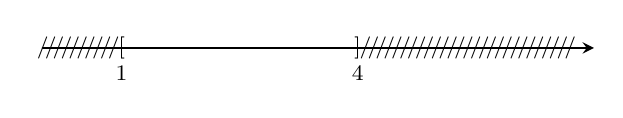
\begin{tikzpicture}[font=\footnotesize,line cap=round,line join=round,thick]
						\node  at (1,0) {$[$};
						 \node at (4,0) {$]$};
						\draw[-stealth]  (0,0)--(1,0) node[below=3pt]{$1$}--(4,0) node[below=3pt]{$4$}--(7,0);
						\foreach \x in {0,.1,.2,...,.9} 
						\draw (\x,0)  node{$/$};
						 \foreach \y in {4.1,4.2,...,6.7}
						\draw (\y,0)  node{$/$};
					\end{tikzpicture}
			\end{center}
			Tập hợp $B$ 
			\begin{center}
				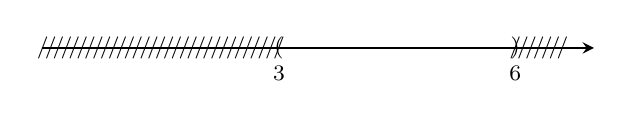
\begin{tikzpicture}[font=\footnotesize,line cap=round,line join=round,thick]
						\node  at (3,0) {$($};
						\node at  (6,0) {$)$};
						\draw[-stealth]  (0,0)--(3,0) node[below=3pt]{$3$}--(6,0) node[below=3pt]{$6$}--(7,0);
						\foreach \x  in {0,.1,.2,...,3}
						\draw  (\x,0) node{$/$};
						 \foreach \y in {6,6.1,...,6.7}
						 \draw (\y,0) node{$/$};
					\end{tikzpicture}
			\end{center}
			\item $A\cup  B = [1;6)$, $A\cap B= (3;4]$.
		\end{enumerate}
	} 
\end{bt}
